\chapter{Карта Лысой и окрестностей}

\begin{center}
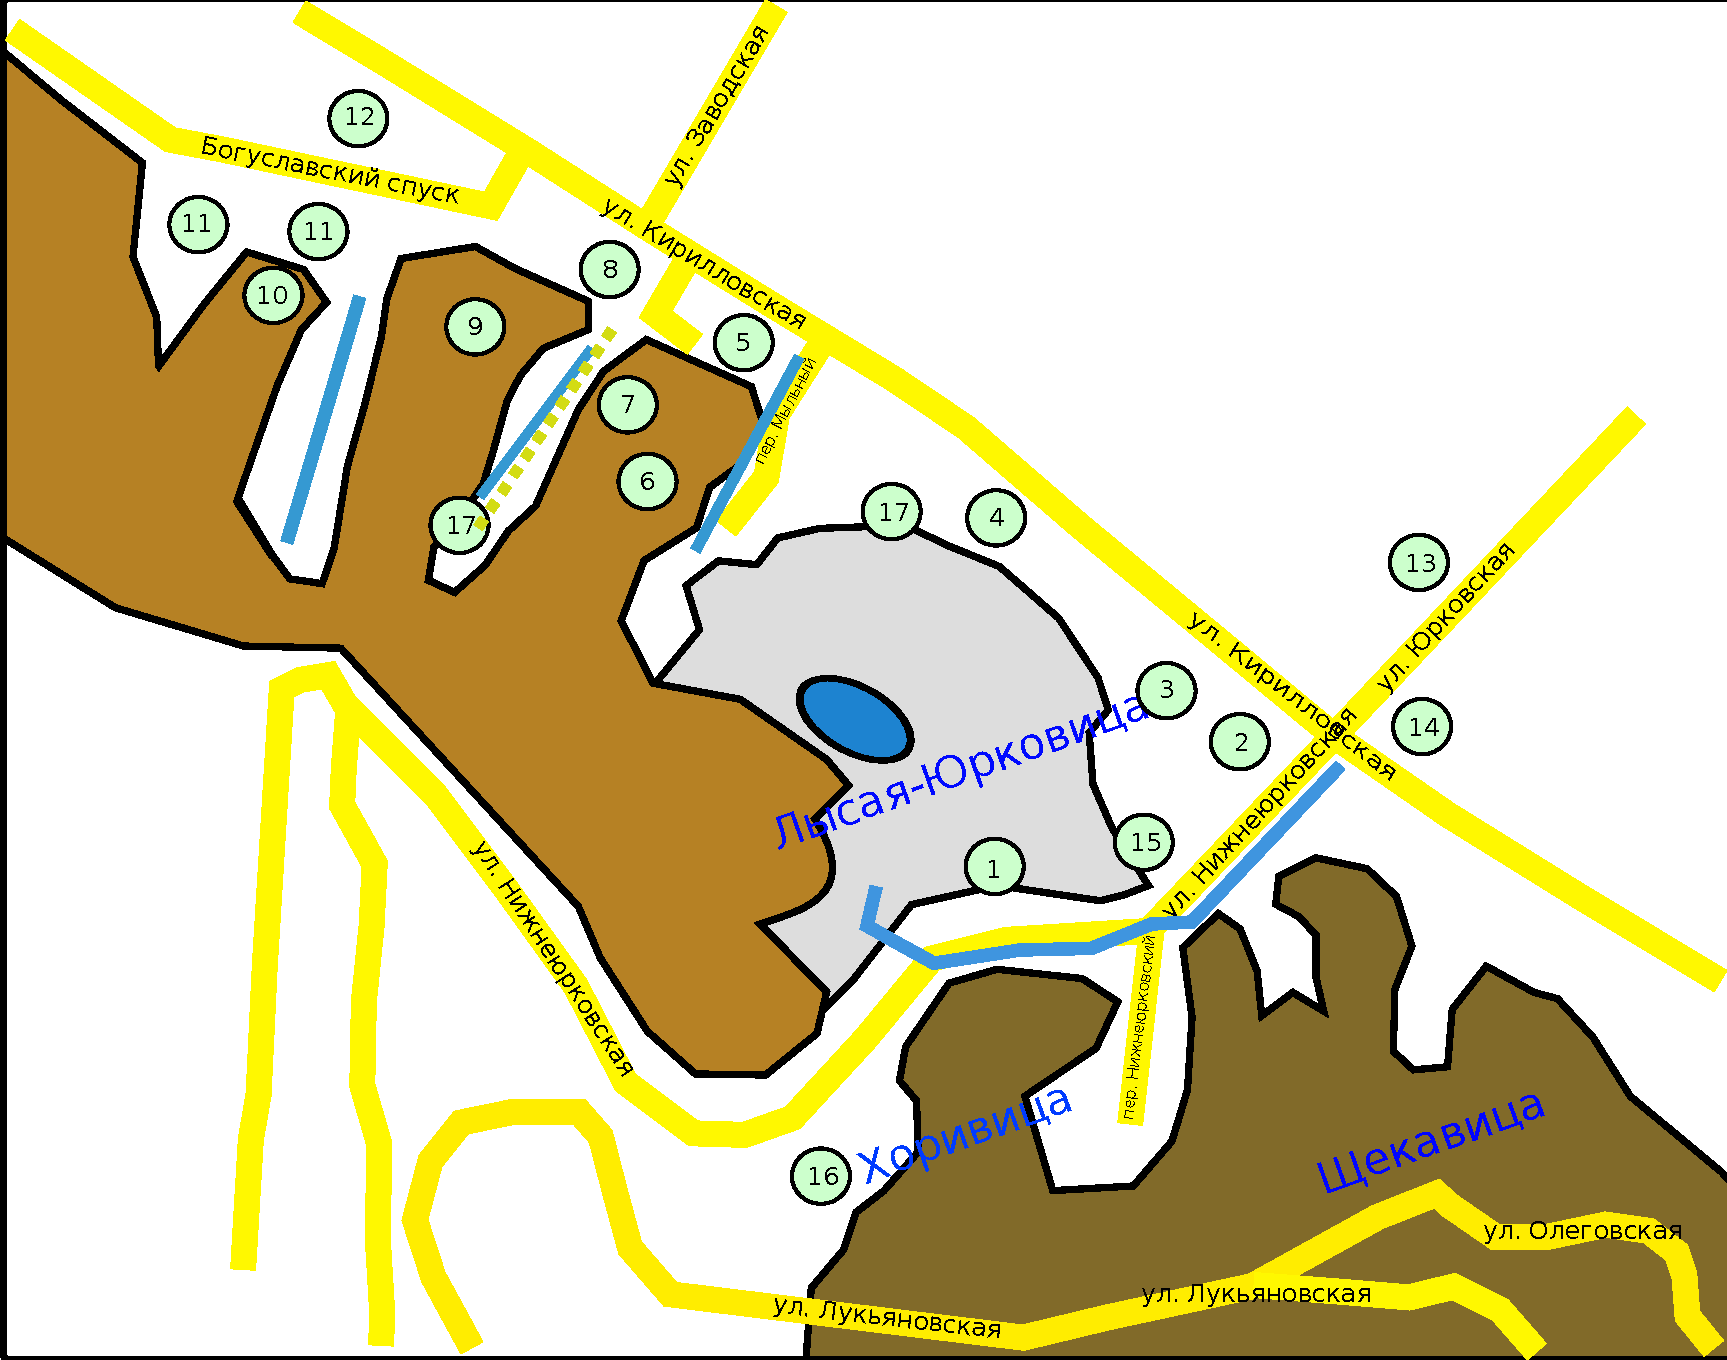
\includegraphics[width=\linewidth]{chast-kirvys/karta/y-main.pdf}
\end{center}

Основные горы подписаны синим. Отдельные объекты на карте обозначены номерами. Это позволило указать историю, что находилось в таком-то месте в разные годы. В следующих главах коснусь каждого объекта подробно, с росписью по годам. Пока же легенда карты в следующем виде – я называю адрес на 2014 год, примерные координаты и последовательно перечисляю, от прошлого к современности (на 2014), что здесь находилось. Адреса по улице Кирилловской во многом сохранились те же, что были до революции 1917 года.

\begin{flushleft}
(1) Нижнеюрковская, 6\\
 50°28'6.66"N 30°29'56.42"E\\
Кирпичный завод киевского гражданина Романовского. Кирпичный завод баронессы Фиркс. Промзона, вч. Склоны оттуда на запад именуются старожилами как Романовщина.

\medskip

(2) Нижнеюрковская, 2\\
50°28'10.74"N 30°30'7.58"E\\ Кирпичный завод Ивана Григоровича. Пивоваренный завод Псиола (Псело). Кирпичный завод Михаила Рихерта. Кирпичный завод. ОАО «Керамблоки».

\medskip

(3) Кирилловская, 35\\
50°28'10.77"N 30°30'2.87"E\\ Пиво-медоваренный завод Псиола (Псело). Пивзавод Михаила Рихерта. Завод Солодовых экстрактов.

\medskip

(4) Кирилловская, 41\\
50°28'18.18"N 30°29'52.56"E\\ Кирпичный завод (не Гудимов, не Рихерта). Металлургическое предприятие. Завод «Общества Киевского пивоваренного завода». Пивзавод №2. «ЗАО Пивзавод на Подоле».

\medskip

(17) Кирпичный завод Шевченко. 1913: адрес Кирилловская, 47. 1914: адрес Верхне-Юрковская, 14

\medskip
 
(5) Кирилловская 51-А, 51/1\\
50°28'23.79"N 30°29'41.2"E\\ Иорданская Димитриевская церковь каменная. Школа. Немецкий концлагерь для воинов Красной Армии. Нотная фабрика. А рядом Кирилловская, 51 – это бывший дом купца Полонника, второй этаж он отдал церкви для проживания священника, теперь в здании – психоневрологический диспансер.\\

\medskip

(6) 50°28'18.38"N 30°29'34.77"E\\
Древние валы и рвы на вершине отрога Лысой горы.\\

\medskip

(7) 50°28'20.75"N 30°29'32.34"E\\
Иорданское кладбище. Уцелевшая часть Иорданского кладбища, находится на большой террасе ниже, северо-западнее пункта 6.\\

\medskip

(8) Кирилловская 53, 55, 57\\
50°28'25.85"N 30°29'35.31"E\\
Винокуренный и дрожжевой завод Марр. Промзона (фабрика молочной кислоты) и пустыри по склону.\\

\medskip

(9) 50°28'23.56"N 30°29'26.12"E\\
«Могилки» из спора 1701 года о разграничении земель, принадлежащих Киеву (магистрату) и Кирилловскому монастырю. Садовое товарищество «Кожевник» (дачи).\\

\medskip

(10) 50°28'23.59"N 30°29'20.42"E\\
Остатки мыса, у которого Викентий Хвойка нашел Кирилловскую стоянку.\\

\medskip

(11) Богуславский спуск 3, 5, 9\\
50°28'26.77"N 30°29'17.4"E\\
Усадьбы Зиваля, Багреева. Усадьбы Зайцева и Бернера. Автобаза.\\

\medskip

(12) 50°28'29.63"N 30°29'26.52"E\\
Усадьбы Зиваля, Багреева. Усадьба Зайцева – еврейская больница Зайцева. Подольский роддом, он же Киевский городской родильный дом №2. Офисные здания «Фармак».\\

\medskip

(13) Юрковская, 3\\
50°28'12.93"N 30°30'13.08"E\\
Древнее каменное здание – остатки его фундамента, фресок, рельефов (и некие захоронения да куски колокола) найдены в 2003 году и соотнесены учеными с церковью 12 века. Дом стыка 19-20 веков, до 1999 года в нем был детский сад, снесен в том же году. Церковь 21 века.\\

\medskip

(14) Юрковская улица, 2-6/32\\
50°28'10.92"N 30°30'13.29"E\\
Старый угловой дом, двухэтажный, где на первом располагался знаменитый магазин «Аполонник» (от владельца лавки и дома, купца Кузьмы Ефимовича Полонника) – последняя вывеска – «Продтовары», рядом в том же доме был «Хлеб», здание снесено в 1986 году. Новый угловой дом.\\

\medskip

(15) Нижнеюрковская 4, 2\\
Кирпичный завод. Кирпичный завод Гудимы. Кирпичный завод Михаила Рихерта. Кирпичный завод. ОАО «Керамблоки».\\

\medskip

(16) Нижнеюрковская 53\\
50°27'57"N 30°29'44"E\\
Котельная «Лукьяновская», Волчий Яр на ряде старых карт.\\

\medskip

(17) Иорданский ручей (исток условен)\\

\medskip
\end{flushleft}

Эта карта понадобится в следующих главах. Мы будем подробно рассматривать её участки. Кроме того, карта полезна для понимания других краеведческих исследований. Она векторная, что позволяет сколь угодно увеличивать масштаб просмотра. 

Карта ориентирована на север и охватывает юг и середину Кирилловских высот. Западная граница Хоривицы отмечена мною условно.  Остальную местность к западу от нее я не рисовал.

Лысая гора, или современная Юрковица – это гора от улицы Нижнеюрковской по отрог (включительно), примыкающий к северо-западу Мыльного переулка. Коричневым цветом я пометил современный рельеф горных отрогов, причем точность соблюдается только включительно по отрог, обозначенный числом 10, однако не западнее его.

Серым цветом, на Лысой горе показаны очертания её склона по состоянию на 1943 год. Там тоже была возвышенность, что видно на аэрофотоснимке того времени. Насколько высокая – я не знаю. По карте 1803 года граница горы еще больше, не столь откушена и начинается почти на одной линии с северным отрогом Щекавицы.

Голубым овалом обозначено карьерное озеро.

Голубые линии – ручьи. Нижний слывет ручьем Юрковицей (показан по состоянию на начало 19 века), его я чуть сместил, чтобы не налезал на улицу. Этим ручьям посвящена отдельная глава. Конечно, они не заканчиваются там, где обрываются на карте, а текут на северо-восток.
 
Переулок от Кирилловской улицы между переулком Мыльным и Богуславским спуском раньше имел название Иорданский и временами соединялся с Мыльным, формой образуя с ним букву П (если смотреть с улицы Кирилловской лицом к горе) с верхней палочкой у подножия склона.

Желтым пунктиром помечена старинная дорога от Иорданского монастыря к Лукьяновке, Старый Никольский ввоз, по выражению Похилевича.

Не следует думать, что раньше разные фабрики стояли по Кирилловской сплошняком – это сейчас промзона довольно плотная, а до революции заводские усадьбы перемежались с обывательскими, жилые дома могли прятаться за промышленными сооружениями, и так далее. Еще в 2014 году на горе над Иорданским переулком были развалины старого жилого домика. В 2015 их отгородили строительным забором. На 2016 год там – остатки развалин и рядом строительство.

На карте внимание уделено объектам по нечетной стороне Кирилловской. Четная, которая у меня белая и пустая, на деле покрыта промзоной.
